\documentclass[border=10pt]{standalone}

\usepackage{tikz}
\usetikzlibrary{calc}

\begin{document}
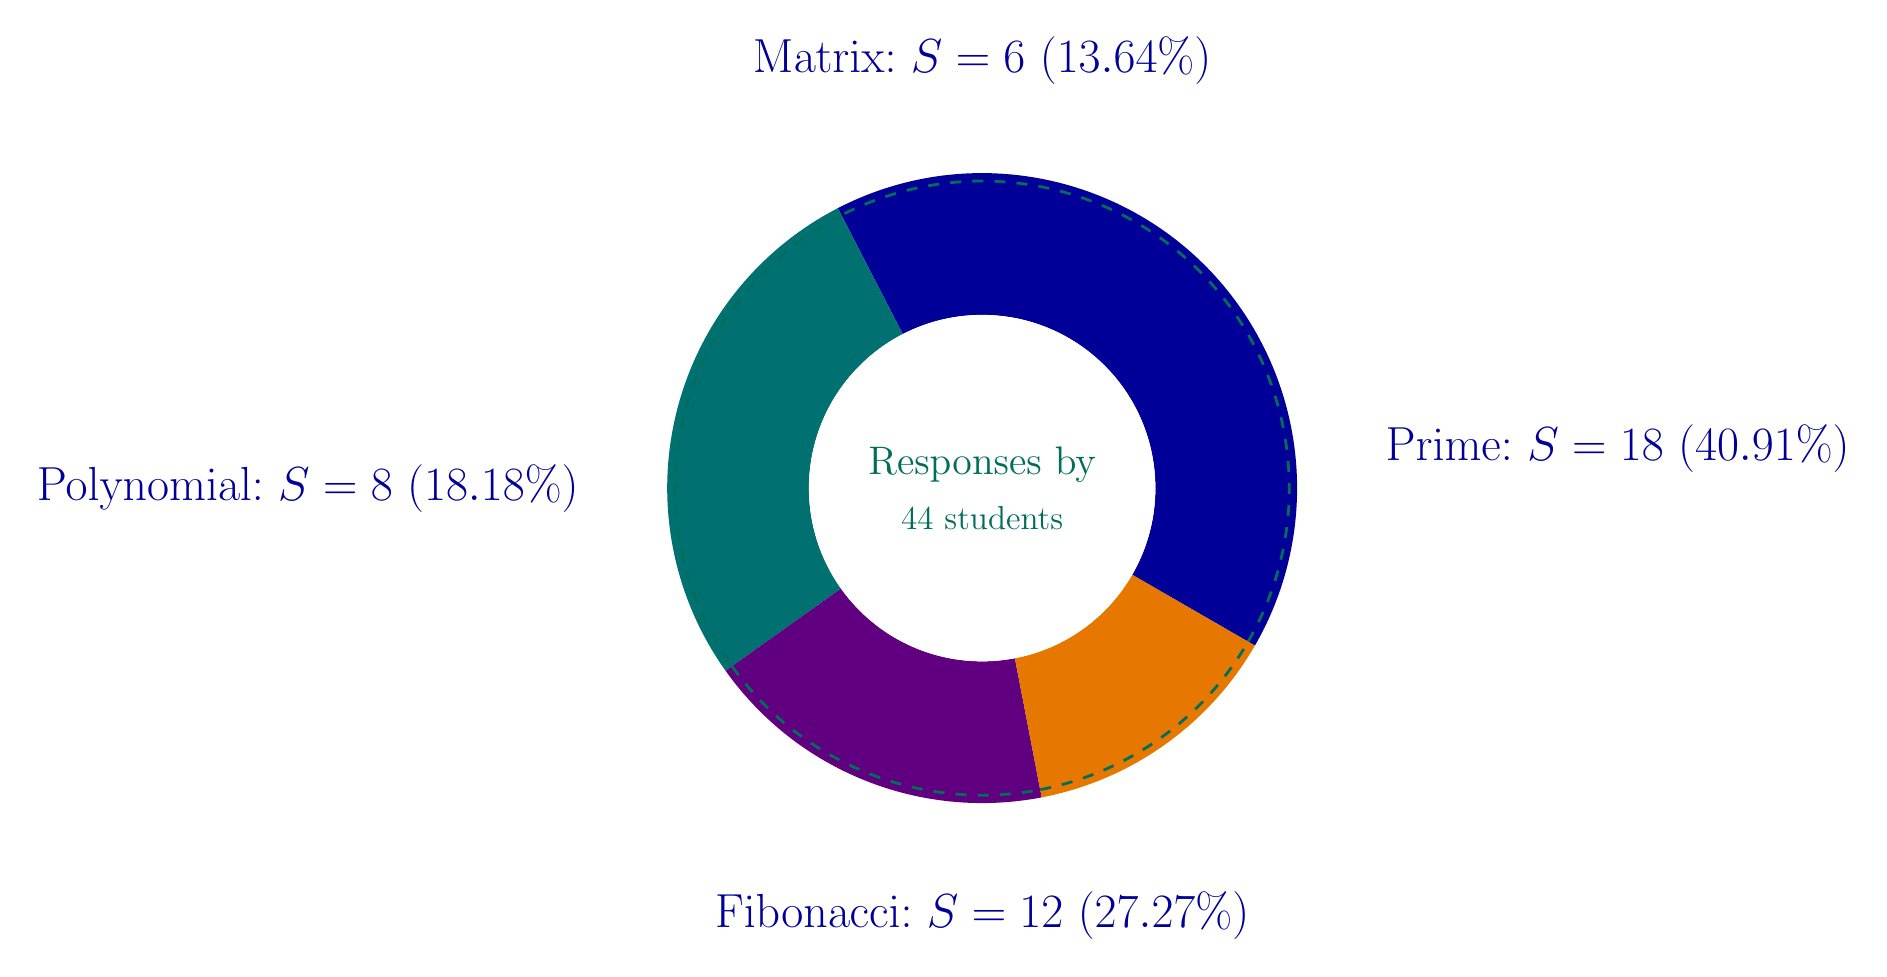
\begin{tikzpicture}[font=\sffamily]

%--- parameters ---------------------------------------------------
\def\Rout{4}    % outer radius
\def\Rin{2.2}   % inner radius (for donut)
\def\Rdash{3.9} % radius of dashed ring
\def\LineWidth{14pt}

% colors (approximate to the figure)
\definecolor{primeblue}{RGB}{0,0,153}
\definecolor{fibgreen}{RGB}{0,112,112}
\definecolor{polyviolet}{RGB}{96,0,128}
\definecolor{matrixorange}{RGB}{230,120,0}
\definecolor{centerteal}{RGB}{0,110,90}

% angles according to values
\def\angPrime{147.27}
\def\angFibo{98.18}
\def\angPoly{65.45}
\def\angMatrix{49.10}

% starting angle (going counter‑clockwise)
\def\start{-30}

% helper macro to draw one annular sector
\newcommand{\annsector}[4]{%
  % #1 = start angle, #2 = end angle, #3 = fill color, #4 = dash color
  \begin{scope}
    \path[draw=none,fill=#3]
      (#1:\Rin) arc (#1:#2:\Rin) --
      (#2:\Rout) arc (#2:#1:\Rout) -- cycle;
    % dashed ring on top
    \path[draw=#4,line width=1pt,dash pattern=on 4pt off 4pt]
      (#1:\Rdash) arc (#1:#2:\Rdash);
  \end{scope}
}

%--- donut sectors (order: Prime, Fibonacci, Polynomial, Matrix) --
\pgfmathsetmacro{\aPrimeStart}{\start}
\pgfmathsetmacro{\aPrimeEnd}{\start+\angPrime}

\pgfmathsetmacro{\aFiboStart}{\aPrimeEnd}
\pgfmathsetmacro{\aFiboEnd}{\aFiboStart+\angFibo}

\pgfmathsetmacro{\aPolyStart}{\aFiboEnd}
\pgfmathsetmacro{\aPolyEnd}{\aPolyStart+\angPoly}

\pgfmathsetmacro{\aMatStart}{\aPolyEnd}
\pgfmathsetmacro{\aMatEnd}{\aMatStart+\angMatrix}

% Draw sectors
\annsector{\aPrimeStart}{\aPrimeEnd}{primeblue}{centerteal}
\annsector{\aFiboStart}{\aFiboEnd}{fibgreen}{centerteal}
\annsector{\aPolyStart}{\aPolyEnd}{polyviolet}{centerteal}
\annsector{\aMatStart}{\aMatEnd}{matrixorange}{centerteal}

%--- inner white circle -------------------------------------------
\fill[white] (0,0) circle[radius=\Rin];

%--- central text -------------------------------------------------
\node[align=center,text=centerteal,font=\Large]
  at (0,0) {Responses by\\[2pt]\large 44 students};

%--- external labels ----------------------------------------------
% Prime (right)
\node[anchor=west,text=primeblue,font=\LARGE]
  at (5.0,0.5) {Prime:~$S = 18\ (40.91\%)$};

% Fibonacci (bottom)
\node[anchor=north,text=primeblue,font=\LARGE]
  at (0,-5.0) {Fibonacci:~$S = 12\ (27.27\%)$};

% Polynomial (left)
\node[anchor=east,text=primeblue,font=\LARGE]
  at (-5.0,0.0) {Polynomial:~$S = 8\ (18.18\%)$};

% Matrix (top)
\node[anchor=south,text=primeblue,font=\LARGE]
  at (0,5.0) {Matrix:~$S = 6\ (13.64\%)$};

\end{tikzpicture}
\end{document}